% Written on Sun Jul 11 17:22:29 CEST 2004 
% by Jean-Baptiste Caillau - ENSEEIHT-IRIT, UMR CNRS 5505
\documentclass[10pt,a4paper]{article}
\usepackage{hyperref}
\usepackage{tikz}
\usepackage{amsmath}
\usepackage{amsthm}
\usepackage{mathrsfs}
\usepackage{graphicx}
\usepackage{color}
\usepackage{multicol}
%\usepackage[french]{babel}
\setlength{\textwidth}{180mm} 
\setlength{\textheight}{280mm} 
\setlength{\topmargin}{-30mm}%{-5mm}
\setlength{\headheight}{2.5mm}
\setlength{\headsep}{7.5mm}
\setlength{\oddsidemargin}{-17mm}%{-10mm}
\setlength{\evensidemargin}{-10mm}
\def\R{\mathbf{R}}
\def\Z{\mathbf{Z}}
\def\N{\mathbf{N}}
\def\W{\mathrm{W}}
\def\L{\mathrm{L}}
\def\C{\mathrm{C}}
\def\H{\mathrm{H}}
\def\HH{\mathscr{H}}
\def\iy{\infty}
\def\t{T}
\def\veps{\varepsilon}
\def\vphi{\varphi}
\renewcommand\vec{\overrightarrow}
\def\co{\mathrm{co}}
\def\cl{\mathrm{cl}}
\def\intr{\mathrm{int}}
\def\Lie{\mathrm{Lie}}
\def\don{\delta_\mathrm{ON}}
\def\doff{\delta_\mathrm{OFF}}
\def\supp{\mathrm{supp}}
\def\Im{\mathrm{Im}}
\def\GL{\mathrm{GL}}
\def\ie{\emph{i.e.}}
\def\cf{\emph{cf.}}
\def\eg{\emph{e.g.}}
\def\apriori{\emph{a priori}}
\def\etc{\emph{etc.}}
\def\noi{\noindent}
\newcommand{\lb}[2]{[#1,#2]}
\def\vect{\mathrm{Vect}}
\def\la{\langle}
\def\ra{\rangle}
\def\tmax{T_\mathrm{max}}
\newtheorem{thrm}{Theorem}[section]
\newtheorem{prpstn}{Proposition}[section]
\newtheorem{lmm}{Lemma}[section]
\newtheorem{crllr}{Corollary}[section]
\theoremstyle{definition}
\newtheorem{dfntn}{Definition}[section]
\newtheorem{rmrk}{Remark}[section]
\begin{document}
\thispagestyle{empty}
% Logos
\noi \begin{tabular}{cccc}
\begin{minipage}[t]{3.6cm} \vspace*{-0.0cm}
\begin{flushleft}

\includegraphics[width=3.6cm]{cfms-2004/logo-mctao2.png}\\
\end{flushleft}
\end{minipage} &
\begin{minipage}[t]{6.0cm} \vspace*{-0.0cm}
\begin{center} 
\includegraphics[width=4.5cm]{cfms-2004/UCA_logo.png}\\
\end{center}
\end{minipage} &
\begin{minipage}[t]{6.0cm} \vspace*{-0.0cm}
\begin{flushright} 

\includegraphics[width=3cm]{cfms-2004/inr_logo_rouge.png}

\includegraphics[width=2.0cm]{cfms-2004/LOGO_CNRS_BLEU.png}
\end{flushright}
\end{minipage}\\
\end{tabular}
\begin{center}
\renewcommand{\thefootnote}{\fnsymbol{footnote}}
{\Large \bf Control of collision orbits \\}
\vspace{0.2cm}
Riccardo Daluiso$^1$, J.B. Caillau$^1$, A. Albouy$^2$
\end{center}
\begin{center}
\begin{multicols}{2}
    \small{$^1$Université Côte d'Azur, CNRS, Inria, LJAD}
    
    \small{$^2$IMCCE, Observatoire de Paris}
\end{multicols}
\end{center}
\noi \begin{tabular}{cc}
\begin{minipage}[t]{20.21cm} \vspace*{-0.0cm} \footnotesize
\noi \textbf{Keywords.} regularization, min time or min fuel
trajectories, collision, control.
\end{minipage}
\end{tabular}
% 1. Orbit transfers
\noi \begin{tabular}{cc}
\begin{minipage}[t]{12.42cm} \vspace*{-0.0cm} \footnotesize
\noi \textbf{1. Regularizations.}
In the $n$-body problem, $n$ point masses move in space under their mutual gravitational interactions as described by Newton's theory of gravity. The forces acting between particles, inversely proportional to the square of the distance between the bodies, approach infinity when the mutual distances approach zero. Therefore, at collision, the equations of motion have singularities. Since Levi-Civita and Sundman, the double collision has been "regularized", \emph{i.e.} the singularity has been made to disappear by means of algebraic transformations. Levi-Civita obtained for the first time in $1904$ a regularizing transformation of the planar restricted 3-body problem based on the map $\mathbf{C} \to \mathbf{C}$,
$z \to z^2$, where the complex plane is the plane of motion. This conformal map sends the orbits of the harmonic oscillator in the ones of the Kepler problem, and was found by Maclaurin in $1742$. This transformation of the coordinates is coupled with a slowing down of the motion by means of the \textit{Sundman reparametization} defined by the differential relation $d\tau = 1/|z| dt$. 
\end{minipage} &
\begin{minipage}[t]{6.0cm} \vspace*{-0.0cm}
\begin{center} \centering 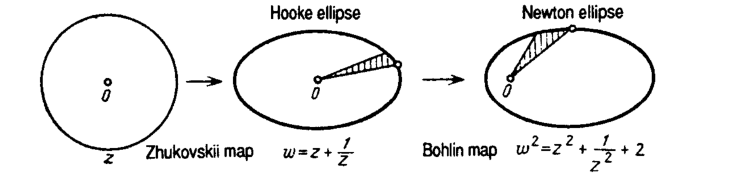
\includegraphics[width=6cm]{cfms-2004/Arnold.png} \end{center}
\emph{Duality between the ellipses of Hooke and Kepler, from the V.I. Arnold's book of $1990$. }
\end{minipage}\\
\end{tabular}
% 2. Min fuel transfer
\noi \begin{tabular}{cc}
\begin{minipage}[b]{7.0cm} \vspace*{0.5cm} \footnotesize
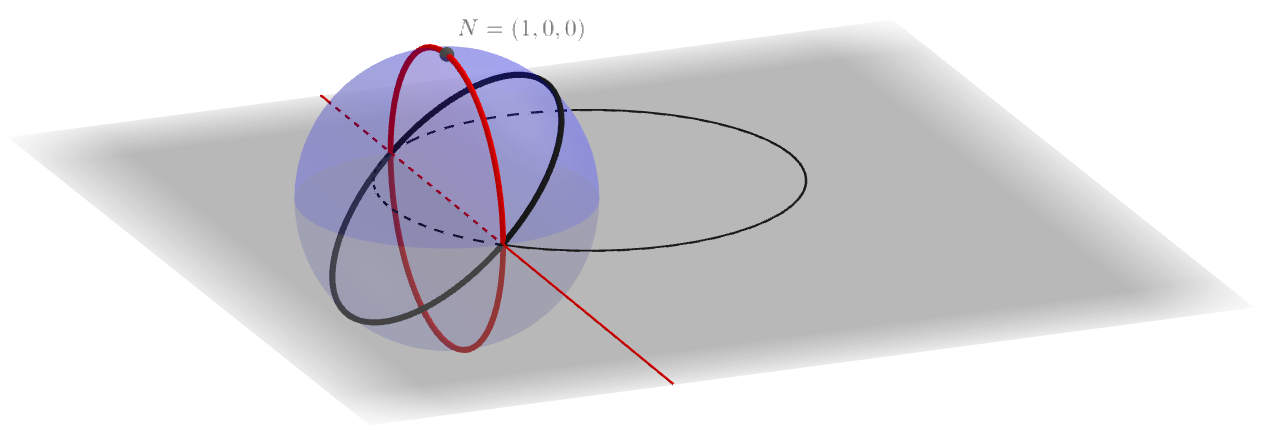
\includegraphics[width=7cm,height=2.4cm]{cfms-2004/proiezione stereografica.png}\\
\noi \emph{Sterographic projections of the great circles correspond to the odographs of Kepelerian velocities. This construction gives rise to the regularisation of Levi-Civita and Moser.}
\end{minipage} &
\begin{minipage}[b]{11.42cm} \vspace*{0.1cm} \footnotesize
\noi \textbf{2.The second Levi-Civita regularization.}
In $1916$ Levi-Civita presented a second regularization of the three-body problem which was ignored by almost all the authors with only a few exceptions. The idea of Levi-Civita was to first regularize a parabolic collision orbit of the Kepler problem by means of the Hamilton-Jacobi method, following procedures from Poincaré. These techniques surprisingly provide contact transformations which make the Hamiltonian of the three-body problem perfectly regular. 
More than fifty years later, Moser $(1970)$ compared the stereographic projection of the great circles of the sphere with Keplerian odograph, following ideas from Fock. This construction gives rise to a compactification of the phase space of the Keplerian orbits for a fixed level of energy together with the same regularization found by Levi-Civita, which is thus designated to be unique and fundamental. We present here these elegant equations:
\[
q \mapsto |p|^2q - 2 \langle  p , q \rangle p, \qquad p \mapsto \frac{p}{|p|^2}.
\]
\end{minipage}\\
\end{tabular}
% 3. Suboptimal trajectories
\noi \begin{tabular}{cc}
\begin{minipage}[b]{11.42cm} \vspace*{0.3cm} \footnotesize
\noi \textbf{3. Application to optimal control.}
Based on classical results, the purpose of the work is the application of the regularization theory to optimal control. We consider the control of a spacecraft under the attraction of one or more bodies, where the control is the thrust, and with the constraint $\int_{0}^{t} f(x,u) \to \textit{min}$ for some function $f$. If $f = 1$, the setting is a time-minimization problem. The equations for the two-body case are $\ddot q  = -\frac{q}{|q|^3} + u$. The \textit{Pontryagin's maximum principle (PMP)} allows us to reduce the differential system to the analysis of an Hamiltonian system for finding optimal solutions. In the most elementary case, we investigate the behaviour of one-dimensional collision orbits, where $q \in \mathbf{R}$ and $u \in [-1,1]$. The extremal trajectories are characterised by piecewise contant controls equal to $\pm 1$. The regularization theory allows the investigation of the motion after the collision with the center of attraction.
\end{minipage} &
\begin{minipage}[b]{7.0cm} \vspace*{0.2cm} \footnotesize
\begin{center} \centering
\begin{tikzpicture}

    % Draw the horizontal line
    \draw[thick] (-2.5,0) -- (2.5,0);
    
    \draw[->] (-1,- 0.3) -- (-0.5, - 0.3);
    
    \node[below] at (-0.8,-0.3) {\small{$u = +1$}};
   
    % Draw the right-to-left arrow above the line
    \draw[->] (1,0.3) -- (0.5,0.3);
    % Label the arrow
    \node[above] at (0.6,0.3) {\small $u = -1$};

    % Define and label the first point (x_0, x'_0)
    \fill (1,0) circle (2pt);
    \node[below] at (1,0) {$(x_0, \dot x_0)$};

    % Define and label the collision point with a sun-like shape
    \draw[fill=yellow] (-1,0) circle (4pt);
    \foreach \angle in {0,45,...,315} 
        \draw[-] (-1,0) -- ++(\angle:6pt);
    \node[above] at (-1,0.3) {};
\end{tikzpicture}
 \end{center}
\emph{\small{One-dimensional collision trajectory with control. After regularizing, the point can bounce at collision and continue the motion in the opposite direction. Extremal trajectories correspond to value of the control equal to $\pm 1$.} }
\end{minipage}\\
\end{tabular}
% 4. Logical constraints
\noi \vspace*{4mm} \begin{tabular}{cc}
\begin{minipage}[b]{7.0cm} \vspace*{0.3cm} \footnotesize
\begin{center} \centering 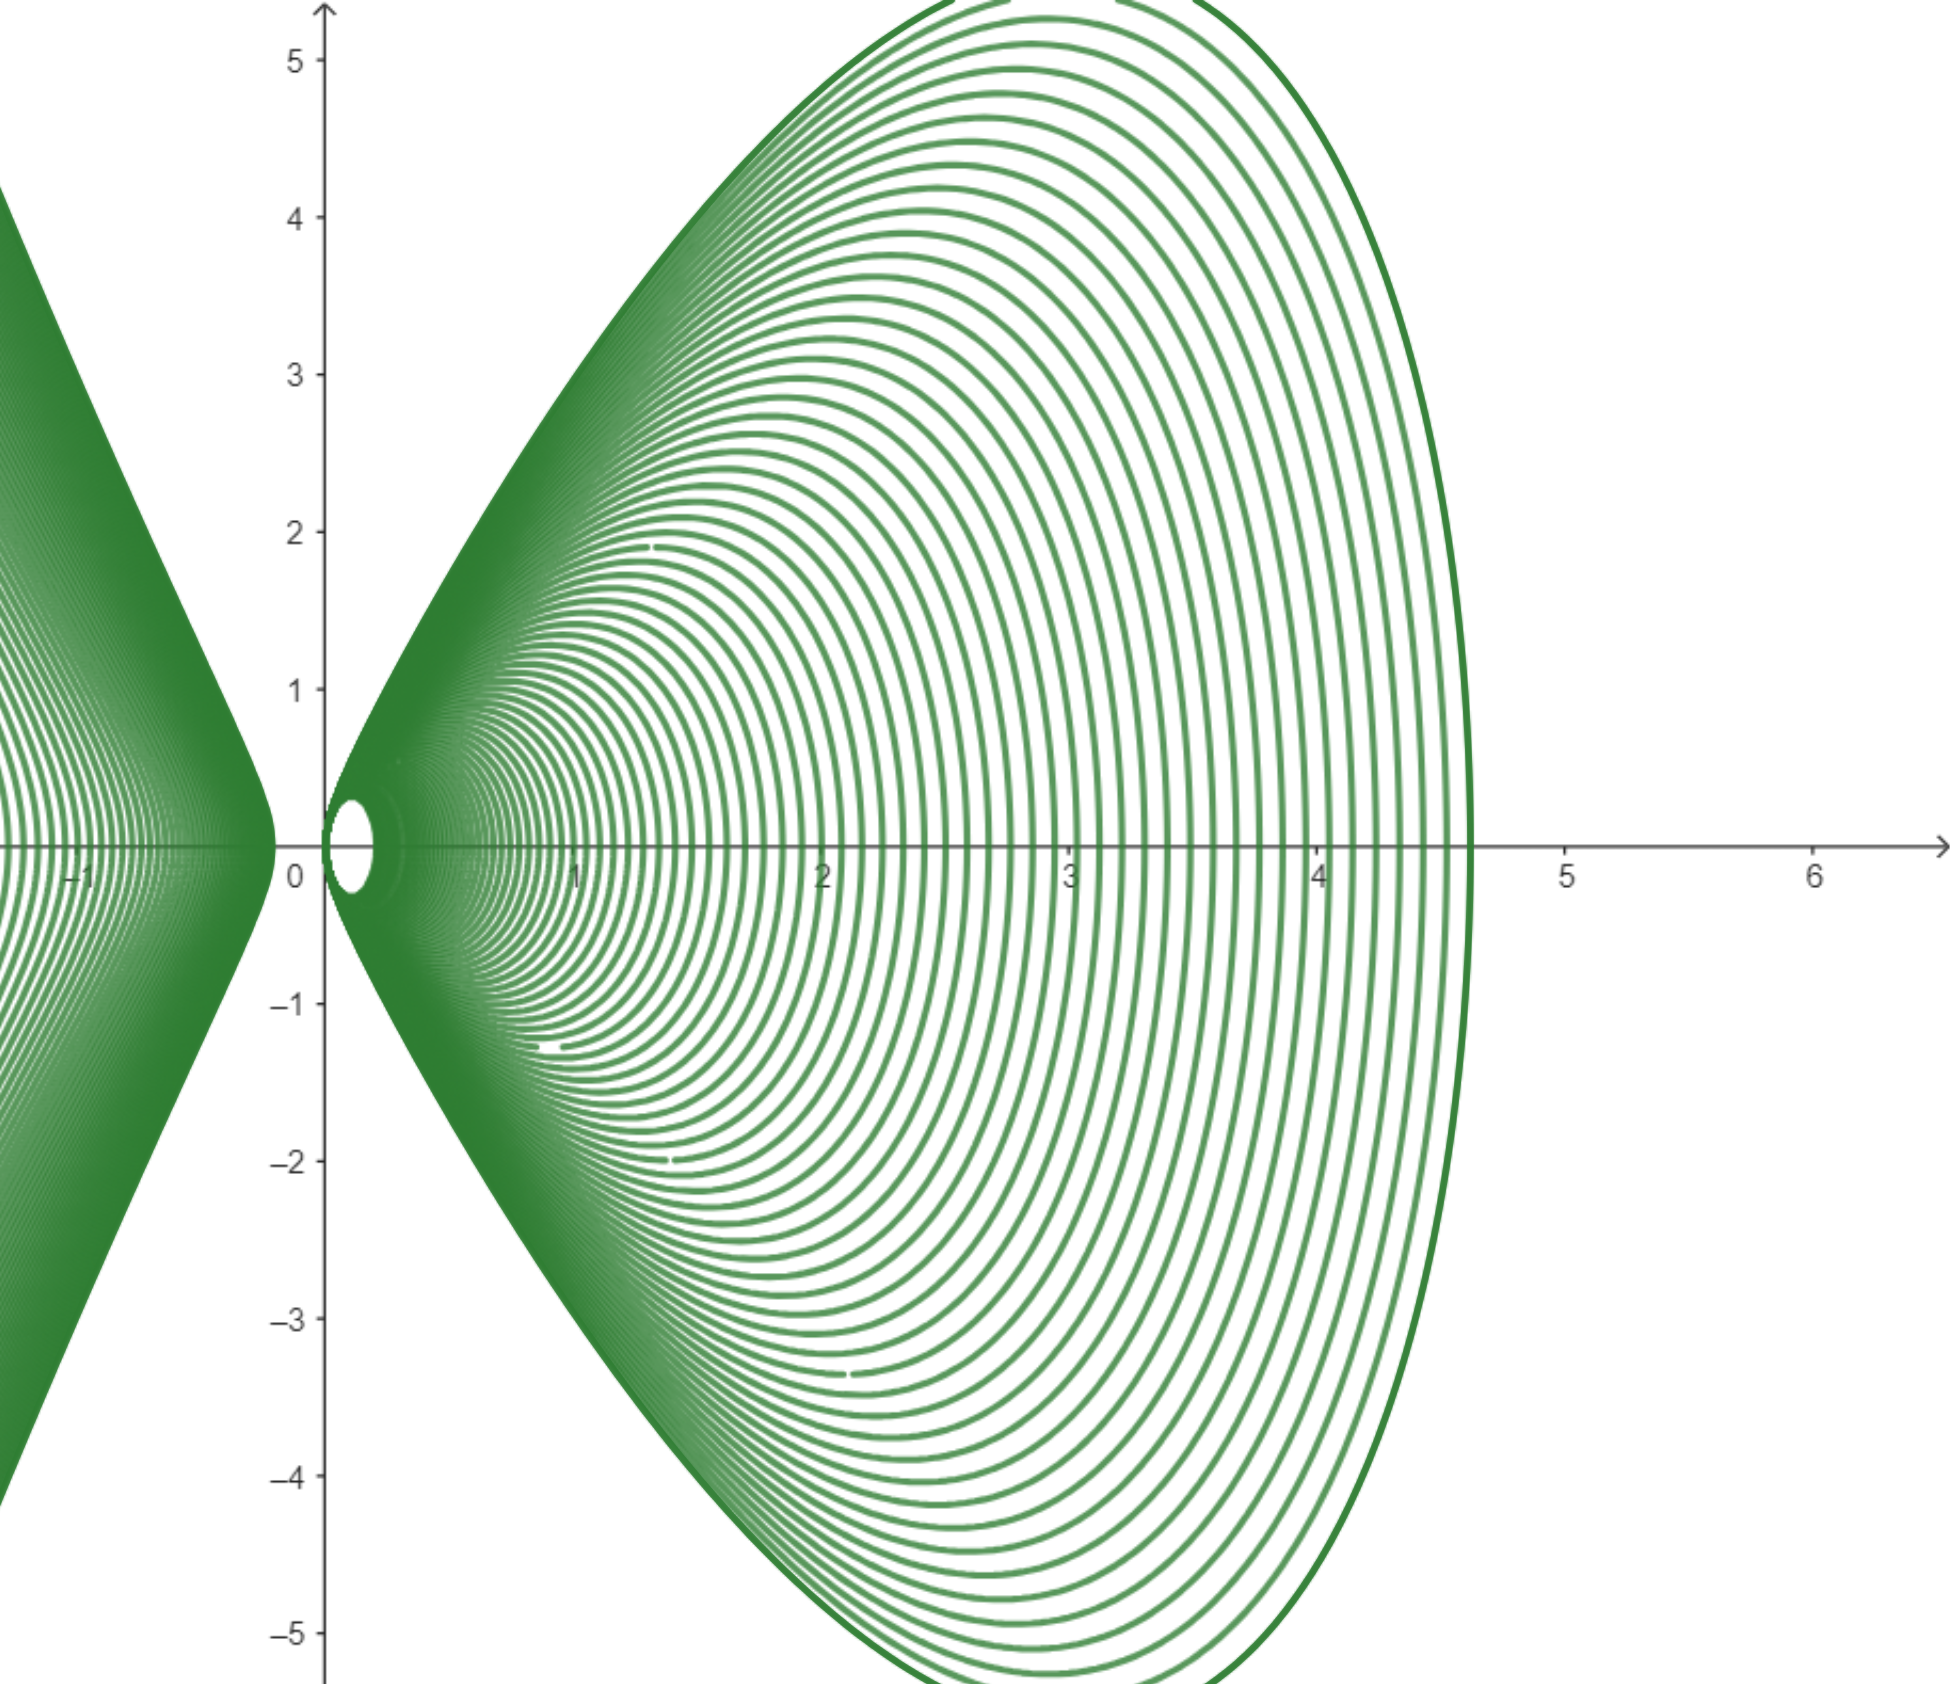
\includegraphics[width=6cm,height=2.3cm]{cfms-2004/phase_space2.png}
\end{center}
\emph{Phase space of the regularized one-dimensional Kepler problem with constant perturbation toward the center of the attraction, $\ddot q = -\frac{1}{q^2} -1$. All the orbits are periodic in the half-plane $x>0$.}
\end{minipage} &
\begin{minipage}[b]{11.42cm} \vspace*{-1cm} \footnotesize
\noi \textbf{4. Future prospects.}
The study of extremal collision trajectories, \textit{i.e} solutions of the PMP, first allows the investigation of the controllability for this type of problem. Further work must be done on the research of optimal trajectories in terms of time or energy minimisation. The problem of planar or spatial collision orbits presents greater difficulties, since the PMP doubles the dimension of the phase space and we need to study equations with singularities in four or six dimensions. Furthermore, an important obstacle in the  theory of regularizations is the the possibility of finding transformations which work for all energy surfaces at the same time, condition which is necessary for the controlled-case since the control perturbation makes the energy non-constant. Given the non-integrability of the controlled Kepler problem even in $2d$, numerical methods will be required to investigate the behaviour of the system.
\end{minipage}\\
\end{tabular}
% References 
\noi \begin{tabular}[ht!]{cc}
\begin{minipage}[t]{9.21cm} \vspace*{-0.0cm} \footnotesize
\noi \textbf{References.}
[1] A. Albouy. , J.~Gergaud and J.~Noailles,
\emph{The Levi-Civita regularizations}, New Frontiers of Celestial
Mechanics: theory and applications, 2023.\\
\noi [2] B. Bonnard, J.B. Caillau, and E. Trélat,
\emph{Geometric optimal control of elliptic Keplerian orbits},
Discrete and Continuous Dynamical Systems - Series S, pp. 929–956, 2005. \\
\noi [3] J.-B. Caillau et al,
\emph{Non-integrability of the minimum-time Kepler problem},
Journal of Geometry and Physics 132, pp. 452–459, 2018.\\
\noi [4] V. Fock,
\emph{Zur Theorie des Wasserstoffatoms},
Z. Physik 98, pp. 145–154, 1935.
\end{minipage} &
\begin{minipage}[t]{9.21cm} \vspace*{-0.0cm} \footnotesize
\noi [5] T. Levi-Civita,
\emph{Regolarizzazione del problema dei tre corpi e sua portata},
Questioni di Meccanica Classica e Relativistica, pp. 1–38, 1924.\\
\noi [6] T. Levi-Civita,
\emph{Sur la r\'egularisation du probl\`em des trois corps},
Rend. Mat. Acc. Lincei 24, 1920.\\
\noi [7] T. Levi-Civita,
\emph{Traiettorie singolari ed urti nel problema ristretto dei tre
corpi},
 Ann. di Mat. Pura ed Appl. (3), 1904. \\
\noi [8] J.K. Moser,
\emph{Regularization of Kepler’s Problem and the Averaging Method
on a Manifold},
Comm. Pure Appl. Math. 23, 1970.
\end{minipage}\\
\end{tabular}
\end{document}


